\documentclass{article}
\usepackage{amsmath}
\usepackage{tikz}
\usetikzlibrary{positioning}

\begin{document}

\begin{figure}[h]
    \centering
    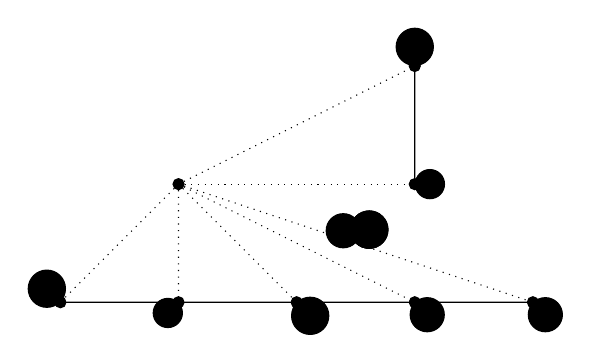
\begin{tikzpicture}[scale=1.5, every node/.style={circle, draw, fill=black, inner sep=0pt, minimum size=4pt}]
        % Define nodes
        \node (a1) at (-1, 0) {};
        \node (b1) at (-2, -1) {};
        \node (c1) at (-1, -1) {};
        \node (d1) at (0, -1) {};
        \node (e1) at (1, -1) {};
        \node (f1) at (2, -1) {};
        \node (g1) at (1, 0) {};
        \node (h1) at (1, 1) {};
        
        % Draw edges
        \draw[dotted] (a1) -- (b1);
        \draw[dotted] (a1) -- (c1);
        \draw[dotted] (a1) -- (d1);
        \draw[dotted] (a1) -- (e1);
        \draw[dotted] (a1) -- (f1);
        \draw[dotted] (a1) -- (g1);
        \draw[dotted] (a1) -- (h1);
        
        \draw (b1) -- (c1);
        \draw (b1) -- (d1);
        \draw (b1) -- (e1);
        \draw (b1) -- (f1);
        \draw (c1) -- (d1);
        \draw (c1) -- (e1);
        \draw (c1) -- (f1);
        \draw (d1) -- (e1);
        \draw (d1) -- (f1);
        \draw (e1) -- (f1);
        
        \draw (g1) -- (h1);
        
        % Label nodes
        \node[above left] at (b1) {$\beta_1$};
        \node[below left] at (c1) {$c_2$};
        \node[below right] at (d1) {$\beta_2$};
        \node[below right] at (e1) {$\alpha_2$};
        \node[below right] at (f1) {$\alpha_3$};
        \node[right] at (g1) {$c_4$};
        \node[above] at (h1) {$\beta_4$};
        
        % Add labels for hyperedges
        \node[above left] at (0.5, -0.5) {$\alpha_4$};
        \node[above right] at (0.5, -0.5) {$\alpha_2$};
        \node[above right] at (0.5, -0.5) {$\beta_3$};
        \node[above right] at (0.5, -0.5) {$\alpha_3$};
        \node[above right] at (0.5, -0.5) {$\beta_1$};
        \node[above right] at (0.5, -0.5) {$\beta_4$};
    \end{tikzpicture}
    \caption{Remaining vertices of the six hyperedges in which Breaker has not yet played in Case 1 of Theorem~\ref{TD(4,4)}. These hyperedges are $\{\alpha_3, \beta_2\}$, $\{c_2, \alpha_2, \beta_2\}$, $\{c_2, \alpha_4, \beta_1\}$, $\{c_3, \alpha_3, \beta_3\}$, $\{c_4, \alpha_2, \beta_3\}$, and $\{c_4, \alpha_4, \beta_4\}$.}
    \label{fig:hyperedges_case1}
\end{figure}

\end{document}